\documentclass{beamer}

\usepackage[utf8]{inputenc}
\usepackage{hyperref}

\usetheme{Berkeley}
\beamertemplatenavigationsymbolsempty
\setbeamertemplate{headline}{}
 
\title{Geo-Visualisierung in FoodChain-Lab}
\date{}
 
\begin{document}
\maketitle
 
\section{1}
\begin{frame}
	\begin{center}
  		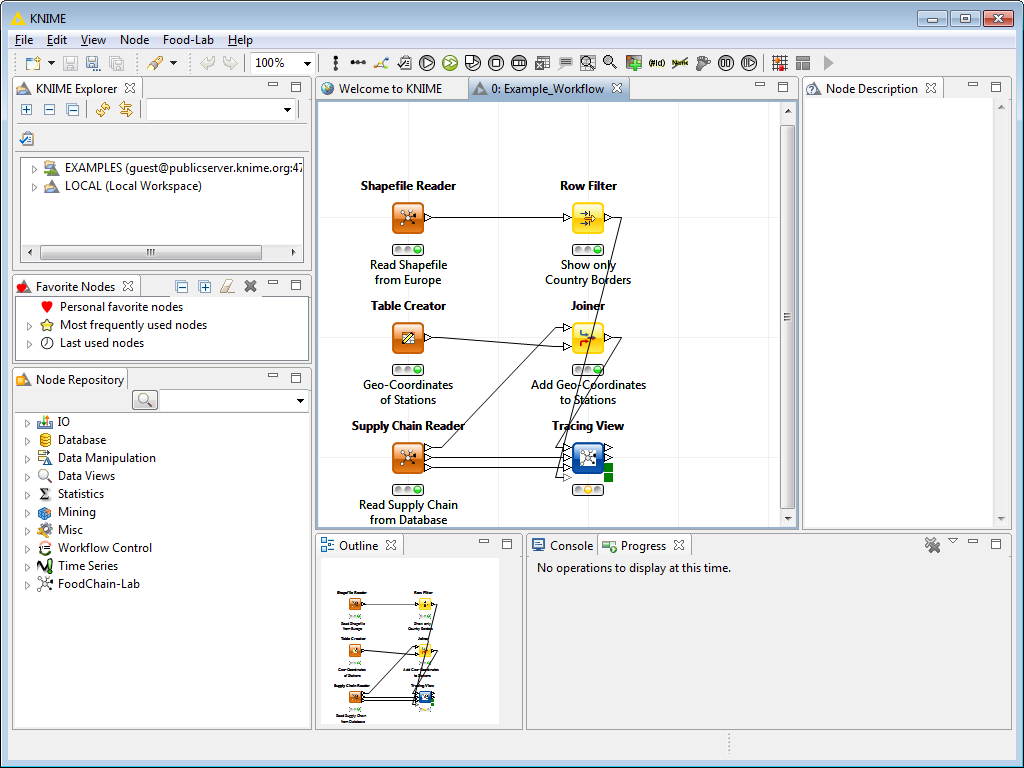
\includegraphics[height=0.6\textheight]{1.png}
	\end{center}
	\begin{itemize}
		\item Importieren sie den Example Workflow von \url{https://github.com/SiLeBAT/BfROpenLabResources/raw/master/GitHubPages/workflows/Example_Workflow.zip}.
		\item Öffnen sie den \textbf{Tracing View} per Doppelklick.
	\end{itemize}
\end{frame}

\section{2}
\begin{frame}
	\begin{center}
  		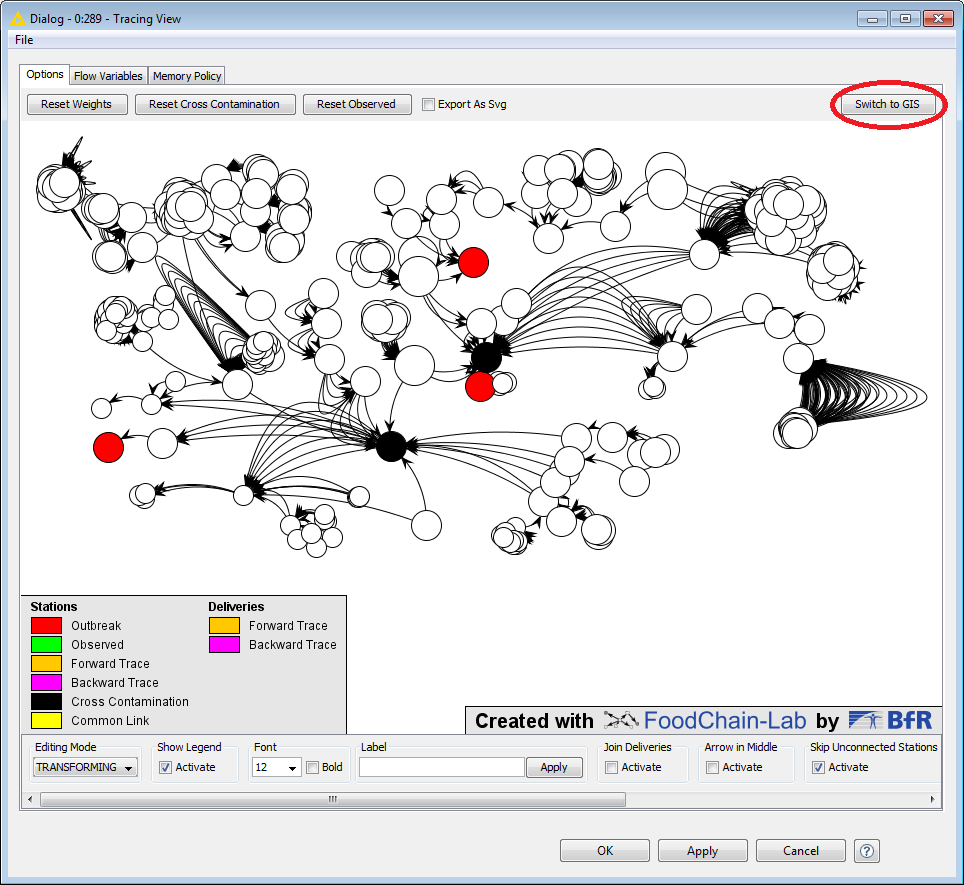
\includegraphics[height=0.6\textheight]{2.png}
	\end{center}
	\begin{itemize}
		\item Nun sehen sie eine graphische Repräsentation des Liefernetzes.
		\item Um zur geographischen Repräsentation zu wechseln wählen sie \textbf{Switch to GIS} rechts oben.
	\end{itemize}
\end{frame}

\section{3}
\begin{frame}
	\begin{center}
  		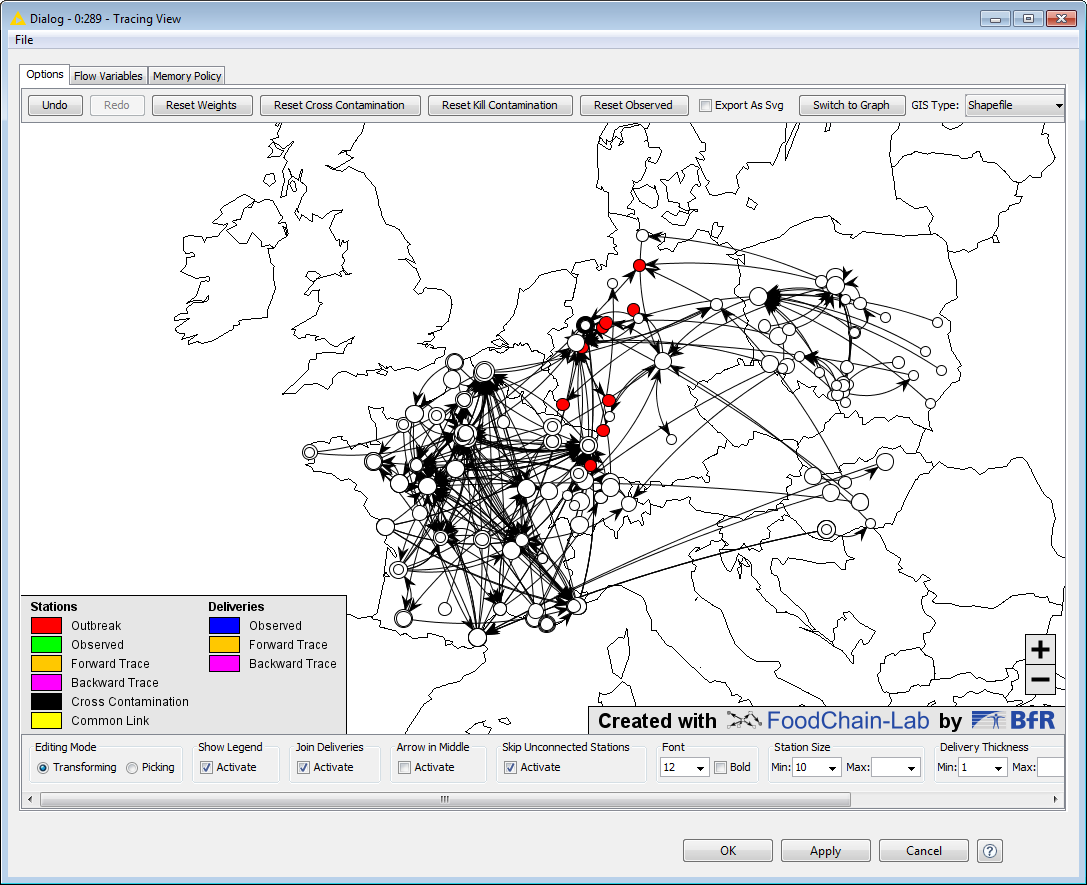
\includegraphics[height=0.6\textheight]{3.png}
	\end{center}
	\begin{itemize}
		\item Um auf auf ein bestimmtes Gebiet zu zoomen wählen sie "TRANSFORMING" als \textbf{Editing Mode} und nutzen sie das Mausrad und die linke Maustaste zum Zoomen und Bewegen des Graphen (funktioniert wie in Google Maps).
	\end{itemize}
\end{frame}

\section{4}
\begin{frame}
	\begin{center}
  		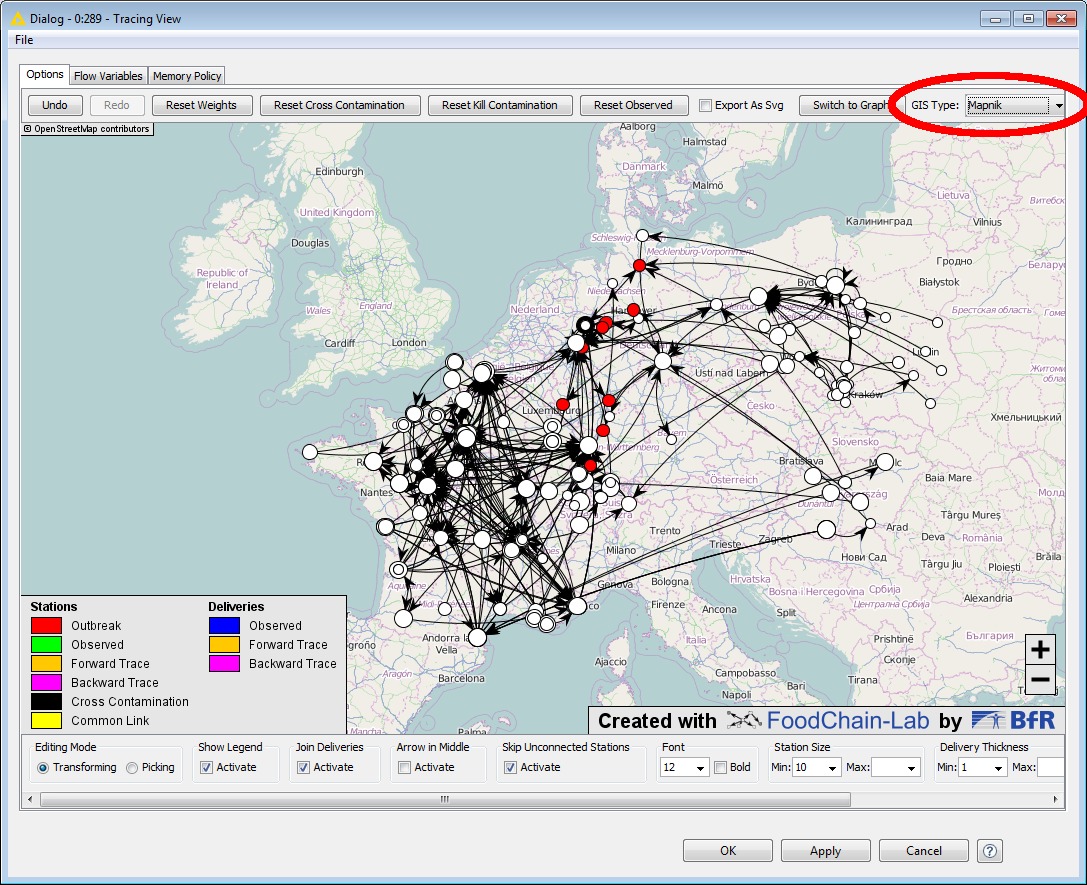
\includegraphics[height=0.6\textheight]{4.png}
	\end{center}
	\begin{itemize}
		\item Hier sehen sie das Liefernetz in Zentraleuropa.
	\end{itemize}
\end{frame}

\section{5}
\begin{frame}
	\begin{center}
  		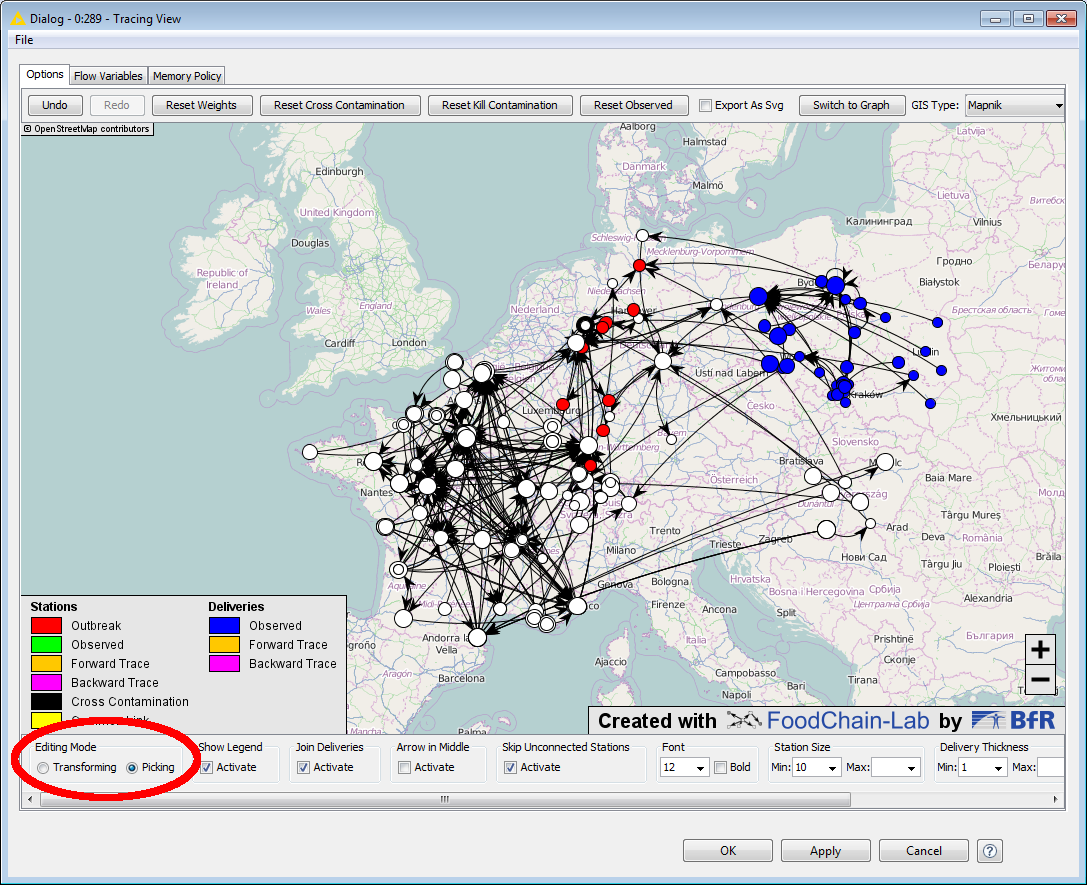
\includegraphics[height=0.5\textheight]{5.png}
	\end{center}
	\begin{itemize}
		\item Wir können nun Station aufgrund ihrer geographischen Lage auswählen.
		\item Setzen sie "PICKING" als \textbf{Editing Mode} and wählen sie alle Stationen in Polen aus, indem sie ein Rechteck um diese Stationen ziehen.
		\item The gewählten Stationen sollten nun blau markiert sein.
		\item Wechseln sie zurück zur graphischen Ansicht, indem sie rechts oben \textbf{Switch to Graph} klicken.
	\end{itemize}
\end{frame}

\section{6}
\begin{frame}
	\begin{center}
  		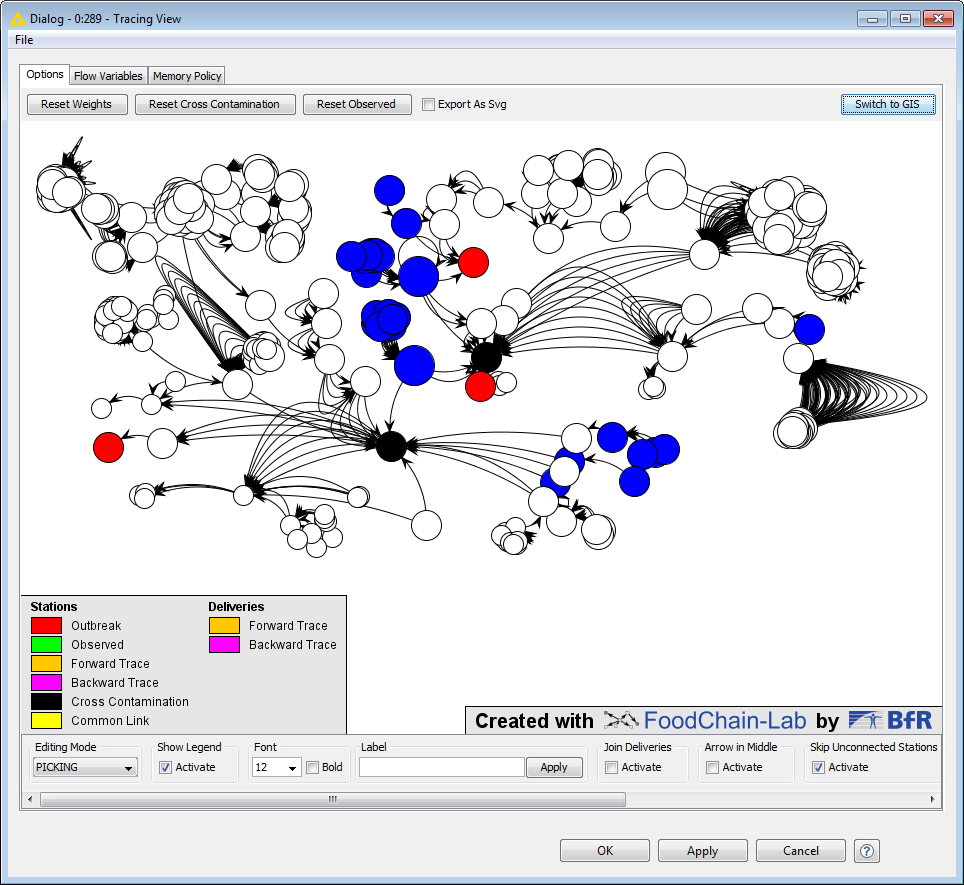
\includegraphics[height=0.5\textheight]{6.png}
	\end{center}
	\begin{itemize}
		\item Die blauen Stationen sind dieselben Stationen, die sie in der geographischen Ansicht ausgewählt haben.
		\item Denn Änderungen, die sie in einer Ansicht machen, werden automatisch auf die andere Ansicht übertragen.
		\item Das macht es einfach zwischen beiden Ansichten hin und her zu wechseln, um die Vorteile der jeweiligen Ansicht zu nutzen.
	\end{itemize}
\end{frame}

\section{7}
\begin{frame}
	\begin{center}
  		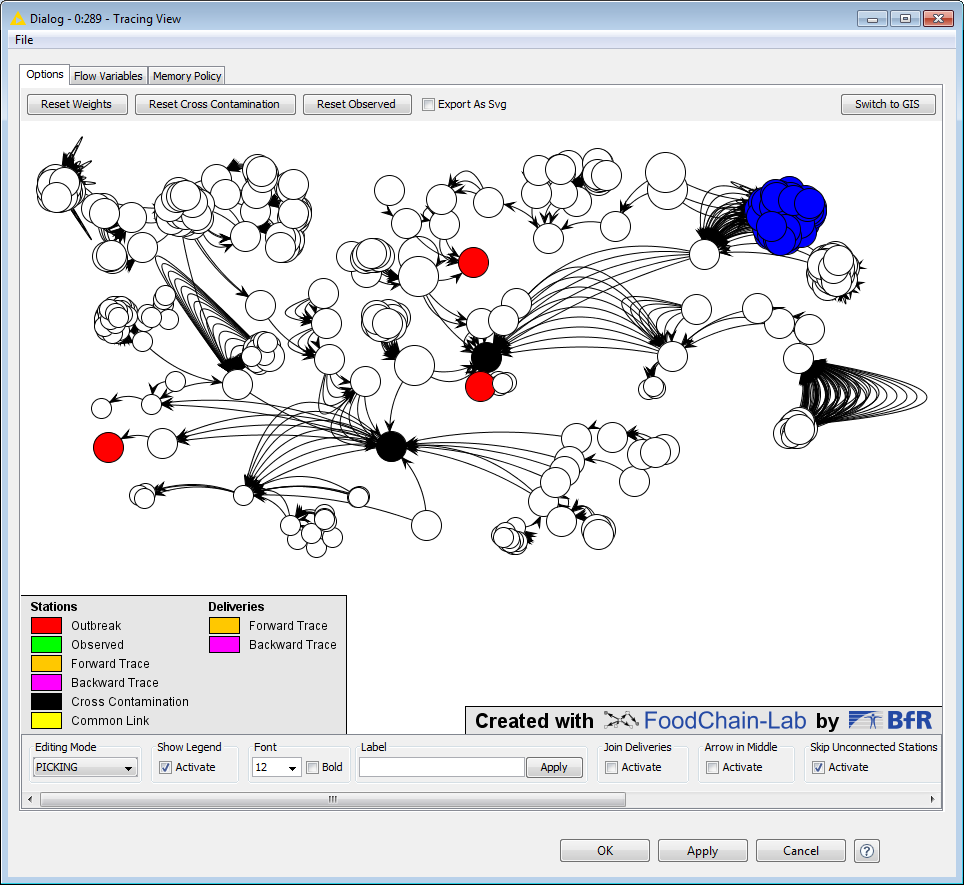
\includegraphics[height=0.6\textheight]{7.png}
	\end{center}
	\begin{itemize}
		\item Nun wählen wir ein "Cluster" von Stationen in der graphischen Ansicht und schauen uns dann die geographische Lage der Stationen an.
		\item Also wählen sie das "Cluster" in der rechten oberen Ecke und klicken sie \textbf{Switch to GIS}.
	\end{itemize}
\end{frame}

\section{8}
\begin{frame}
	\begin{center}
  		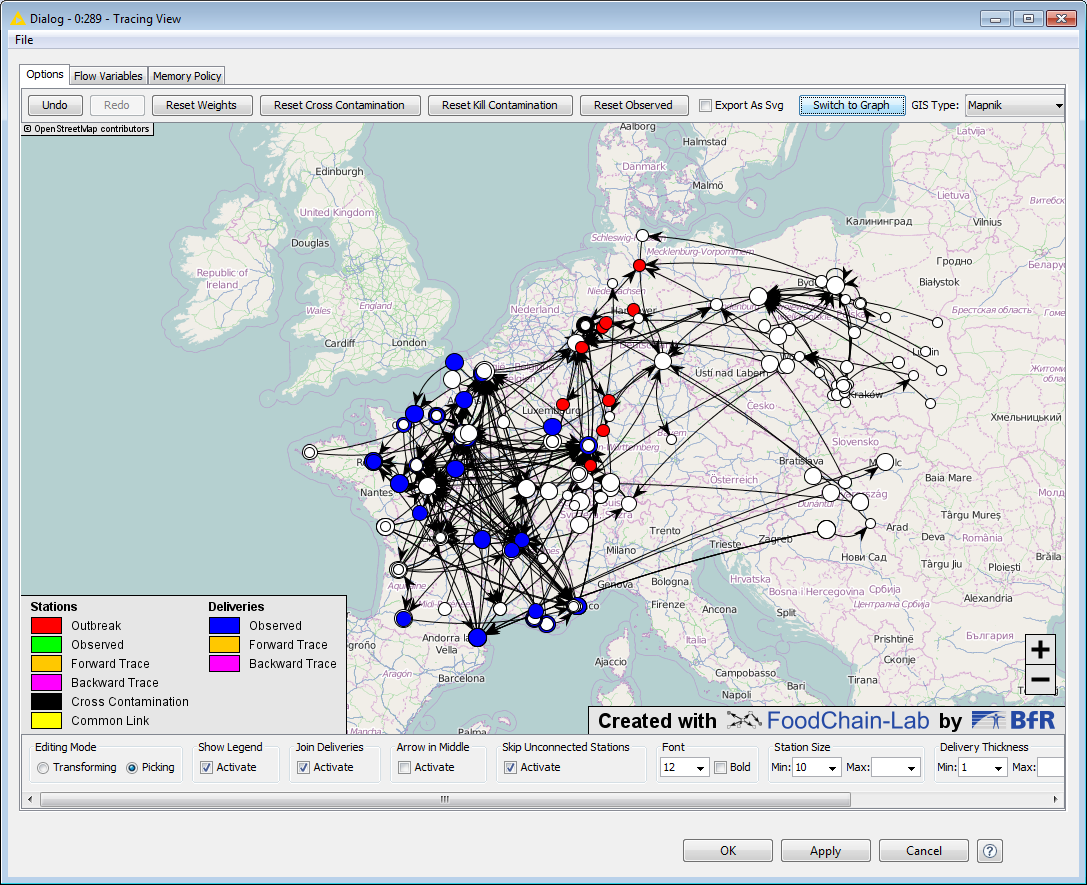
\includegraphics[height=0.6\textheight]{8.png}
	\end{center}
	\begin{itemize}
		\item Wie sie sehen, sind die Stationen des Clusters über Frankreich verteilt.
	\end{itemize}
\end{frame}

\end{document}